\documentclass[paper=a4, fontsize=12pt]{scrartcl} % A4 paper and 11pt font size

\usepackage[T1]{fontenc} % use 8-bit encoding that has 256 glyphs
\usepackage{fourier}     % use the Adobe Utopia font for the document
                         % (comment this line to return to the LaTeX default)
\usepackage[english]{babel} % English language/hyphenation
\usepackage{amsmath,amsfonts,amsthm} % math packages
\usepackage{subeqnarray}
\usepackage{manfnt}
\usepackage{lipsum} % used for inserting dummy 'Lorem ipsum' text into the template
\usepackage{bold-extra}
\usepackage{bclogo}
\usepackage{listings}
\usepackage[utf8]{inputenc}
\usepackage{amsthm}
\usepackage{amssymb}
% default fixed font does not support bold face
\DeclareFixedFont{\ttb}{T1}{txtt}{bx}{n}{11} % for bold
\DeclareFixedFont{\ttm}{T1}{txtt}{m}{n}{11}  % for normal

% custom colors
\usepackage{color}
\definecolor{deepblue}{rgb}{0,0,0.5}
\definecolor{deepred}{rgb}{0.6,0,0}
\definecolor{deepgreen}{rgb}{0,0.5,0}
\definecolor{lightblue}{rgb}{0.95,0.95,1}
\definecolor{lightgrey}{rgb}{0.6,0.6,0.6}
\usepackage{listings}

% use graphics packages
\usepackage{graphicx}
\usepackage{float}
\usepackage{tikz}
\usetikzlibrary{matrix}
\usetikzlibrary{calc}
\usetikzlibrary{patterns,fadings}

\graphicspath{ {images/} }
\newenvironment{claim}[1]{\par\noindent\underline{Claim:}\space#1}{}
\newenvironment{claimproof}[1]{\par\noindent\underline{Proof:}\space#1}{\hfill $\blacksquare$}
% python style for highlighting
\newcommand\pythonstyle{\lstset{
language=Python,
backgroundcolor=\color{lightblue},
basicstyle=\ttm,
    % add keywords here
keywordstyle=\ttb\color{deepblue},
emph={while,for,if,elif,else,def,as,shape,conj,dot,copy,flatten,eye,zeros,ones,hstack,vstack,real,imag,conjugate,sin,cos,exp,append,insert,index,__main__}, % custom highlighting
%emphstyle=\ttb\color{deepred},     % custom highlighting style
emphstyle=\ttb\color{deepblue},     % custom highlighting style
stringstyle=\color{deepgreen},
commentstyle=\color{lightgrey},
frame=tb,                         % any extra options here
numbers=left,
showstringspaces=false            %
}}

% python environment
\lstnewenvironment{python}[1][]
{
\pythonstyle
\lstset{#1}
}
{}

% python for external files
\newcommand\pythonexternal[2][]{{
\pythonstyle
\lstinputlisting[#1]{#2}}}

% python for inline
\newcommand\pythoninline[1]{{\pythonstyle\lstinline!#1!}}


\usepackage{sectsty}        % allows customizing section commands
\allsectionsfont{\centering \normalfont\scshape}      % make all sections centered
                                                      % the default font and small caps

\usepackage{fancyhdr}        % custom headers and footers
\pagestyle{fancyplain}       % makes all pages in the document conform to
                             % the custom headers and footers
\fancyhead{}                 % no page header - if you want one, create it in
                             % the same way as the footers below
\fancyfoot[L]{}              % empty left footer
\fancyfoot[C]{}              % empty center footer
\fancyfoot[R]{\thepage}      % page numbering for right footer
\renewcommand{\headrulewidth}{0pt}     % remove header underlines
\renewcommand{\footrulewidth}{0pt}     % remove footer underlines
\setlength{\headheight}{13.6pt}        % customize the height of the header

\numberwithin{equation}{section}       % number equations within sections
                                       % (i.e. 1.1, 1.2, 2.1, 2.2 instead of 1, 2, 3, 4)
\numberwithin{figure}{section}         % number figures within sections
                                       % (i.e. 1.1, 1.2, 2.1, 2.2 instead of 1, 2, 3, 4)
\numberwithin{table}{section}          % number tables within sections
                                       % (i.e. 1.1, 1.2, 2.1, 2.2 instead of 1, 2, 3, 4)

\setlength\parindent{0pt}         % removes all indentation from paragraphs
                                  % comment this line for an assignment with lots of text

%--------------------------
%	TITLE SECTION
%--------------------------

\newcommand{\horrule}[1]{\rule{\linewidth}{#1}} % create horizontal rule command
                                                % with 1 argument of height

\title{
\normalfont \normalsize
\textsc{Imperial College London, Department of Mathematics} \\ [25pt]
\horrule{0.5pt} \\[0.4cm]                      % thin top horizontal rule
\huge Scientific Computing (M3SC) Project 2 \\           % the assignment title
\horrule{2pt} \\[0.5cm]                        % thick bottom horizontal rule
}

\author{Omar Haque}
\date{\normalsize\today}

\begin{document}
%\ttfamily
%\fontseries{b}\selectfont

\maketitle

\section{Solution Strategy}

In this coursework, I will use the algorithmic steps provided to design a workflow and job schedule that minimises the duration of the processes while maximising the number of processes that can be executed in parallel. \\
Rather than describing a strategy in one section and providing the implementation in another, I will be running through each of the steps and describing the functions used in chronological order, finishing on the main code.
\subsection{Extract data}
In order to make this program as robust and as general as possible, I have written a csv file which contains the data from Table 1.1 of the question, i.e the List of jobs, their duration and dependencies.
The function \textit{extract\_data} uses the csv module to iterate through every row of the datafile, and combine them into a numpy array.

\begin{python} 
import csv
import numpy as np
import sys


def extract_data(file_name):
    """
    This function uses the csv module to extract the 'jobs', 'durations'
    and 'has to be completed before' columns

    :param file_name: a csv file containing the data
    :return: a total_nodesx3 np.array containing the 'jobs', 'durations'
    and 'has to be completed before' columns
    """
    # e.g. file_name = './data/jobslist'
    job = []
    duration = []
    completed_before = []

    # open the file
    with open(file_name, 'r') as file:

        AAA = csv.reader(file)
        # iterate through each row
        for i, row in enumerate(AAA):
            # add the job number
            job.append(int(row[0]))
            # add the duration
            duration.append(int(row[1]))
            # if there are jobs to be completed before, add them
            if len(row) > 2:
                completed_before.append([int(node) for node in row[2:]])

            else:
                # else add an empty list. 
                completed_before.append([])

    file.close()

    # combine these together
    data_frame = np.column_stack((job, duration, completed_before))

    return data_frame
    \end{python}


Running this code then produces the array shown in figure \ref{data}
\begin{python}
data = extract_data('./data/jobslist')
\end{python}

\begin{figure}[t]\label{data}
\caption{np.array produced from extract\_data}
\centering
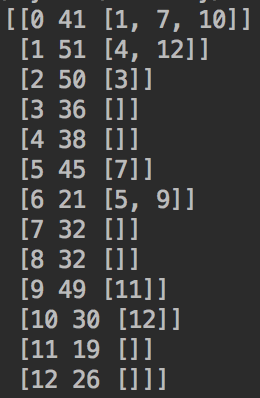
\includegraphics{data}
\end{figure}

\subsection{Constructing the graph}
We now construct the directed graph, as described in steps \textbf{1,2,3} and \textbf{4} of algorithm 1.1 in the question. For job $m \in \{ 0,1,\dots, 12 \}$ I write $m_{s}$ and $m_{f}$ to mean the start and finish node for job m respectively. I also write $v_{s}$ and $v_{f}$ to mean the virtual start and virtual finish node respectively.

I will construct an adjacency matrix, $W = \{ w_{i,j} \}$, where $w_{i,j}$ denotes the edge weight between node $i$ and node $j$. The ordering of the matrix rows and columns is the following sequence $$ 0_{s} 1_{s} \dots 12_{s} 0_{f} 1_{f} \dots 12_{f} v_{s} v_{f}$$
The weights $w_{i,j}$ are specified by steps \textbf{1,2,3} and \textbf{4} of algorithm 1.1, I write the conditions here. $\forall$ jobs m,n $\in \{ 0,1,\dots 12\}$:
\begin{itemize}
  \item $w_{m_{s},m_{f}}$ = the duration of job m. By inspection, the duration of a job is always strictly positive.
  \item $w_{m_{f},n_{s}}$ = 0 if job m has to be completed before job n.
  \item $w_{v_{s},m_{s}} = 0$
  \item $w_{m_{f},v_{f}} = 0$
\end{itemize}

Else, we take a value of $w_{i,j} = -1$ if node $i$ is not connected to node $j$. 

Here is the python implementation:

\begin{python}
def generate_weight_matrix(data):
    """
    This function uses the data to create an adjacency matrix, based
    on the rules outlined.

    :param data: three column np.array with 'jobs', 'durations'
    and 'has to be completed before' columns
    :return: the adjacency matrix for this graph
    """
    global total_nodes, virtual_start, virtual_finish,job_duration
    # we start with an array of -1s and populate the entries that
    # correspond to connected nodes.
    total_nodes = data.shape[0]
    weight_matrix = -1 * np.ones((2 * total_nodes + 2, 2 * total_nodes + 2)
                                 , dtype=int)

    # node start is the index of start jobs
    node_start = data[:, 0].astype(int)
    # job_duration are the job durations for each job
    job_duration = data[:, 1].astype(int)

    # joining each node start to node finish, with the weight as that job's
    # duration.
    weight_matrix[node_start, node_start + 13] = job_duration

    # note on efficiency: I could perhaps do the following for
    # loop by flattening the data[:,2] column, but I need to
    # create a list of node_start corresponding to the number of
    # jobs that each job depends on. This is O(N) anyway, so doing
    # this via a for loop isn't slower.

    # note: also, python doesn't like slicing like a[0,[[4,5],[1,2,3]]]

    for row in data:
        jobs2 = row[2]
        node_start2 = row[0]
        for job in jobs2:
            # this is the connections of dependent jobs
            weight_matrix[node_start2 + 13, job] = 0

    # these are the indices for virtual start and finish
    virtual_start = int(weight_matrix.shape[0]) - 2
    virtual_finish = int(weight_matrix.shape[0]) - 1

    # allow movement between virtual start and all the nodes
    weight_matrix[virtual_start, 0:total_nodes] = 0
    # allow movement from all the nodes to virtual finish
    weight_matrix[total_nodes:virtual_start, virtual_finish] = 0

    return weight_matrix
\end{python}

Running this with the data gives us our adjacency matrix, $W$.

\begin{python}
weights = generate_weight_matrix(data)
\end{python}

\subsection{Finding the longest path}

We wish to determine the longest path from virtual start to virtual finish. Clearly, the longest path in $W$ is the shortest path in the graph defined by $A:=-W$, where $A = \{a_{i,j} \}$. If we look at the definition of W in section 1.2, we see that node $i$ is connected to node $j$ $\iff$ $w_{i,j} \geq 0 \iff a_{i,j} \leq 0$, since $w_{i,j} = -a_{i,j}$. Similarly, node $i$ is not connected to node $j \iff w_{i,j} = -1 \iff a_{i,j} = 1$. \\
Therefore to find the shortest path in A from $v_{s}$ to $v_{f}$ we can apply the Bellman Ford algorithm (since we have negative weights), with the modification that instead of a weight of 0 implying two nodes are not connected, we use 1 instead. I outline these changes below:

\begin{figure}[h]
\caption{changes to the Bellman Ford algorithm}
\centering
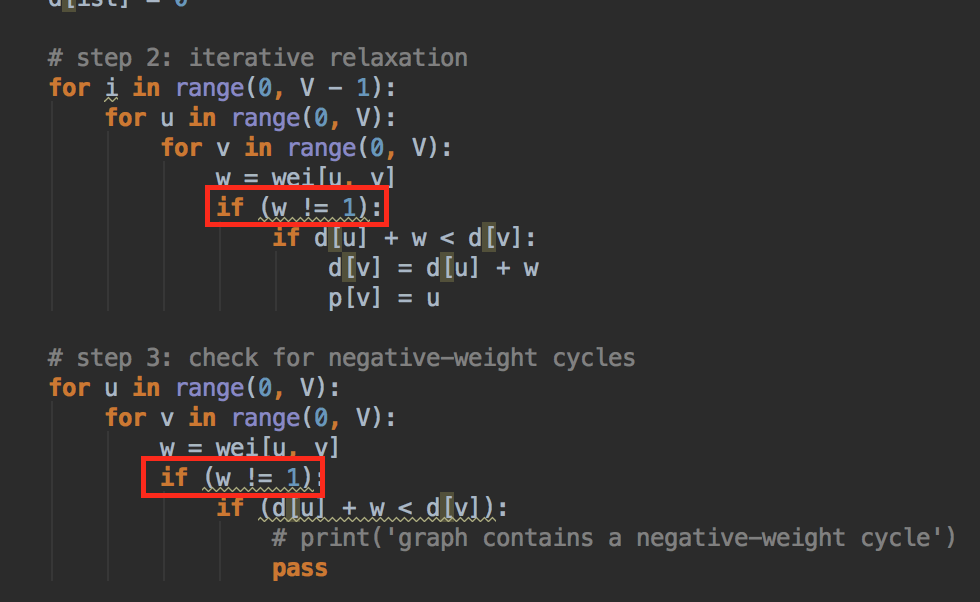
\includegraphics{changes}
\end{figure}

Otherwise, the code is the same as from tutorials, so I will not include it in full here.\\ \\
The following code calculates the longest path from $v_{s}$ to $v_{f}$.

\begin{python}
    adjusted_weights = -1 * weights
    longest_path = updated_bellman_ford(
        virtual_start, virtual_finish, adjusted_weights)[1:-1:2]
\end{python}
printing this longest path gives:
\begin{figure}[h]
\caption{longest path from virtual start to virtual finish}
\centering
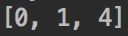
\includegraphics[scale=0.9]{long}
\end{figure}

\bcattention \quad since our adjacency matrix uses the ordering $0_{s} 1_{s} \dots 12_{s} 0_{f} 1_{f} \dots 12_{f} v_{s} v_{f}$, our output will follow the same style. i.e $[v_{s},node1_{s},node1_{f},node2_{s},node2_{f},\dots,nodek_{s},nodek_{f},v_{f}]$. But the virtual nodes are just dummy nodes. We're really trying to find the longest dependent job sequence, and they ensure that we have. So we need to bring our results back to the normal scale, by removing the first and last values, then taking every second value. The python slice [1:-1:2] does exactly this. \\ \\

So $0 \to 1 \to 4$ is the longest string of jobs.

\subsection{Finding the earliest start and stop times}
In this section, we adopt the following notation. For a job $m \in \{0,1,\dots,12 \}$, we write $b_{m}$ for the path 
$$ b_{m} = m_{s} \to m_{f} $$

The first thing to realise is that the earliest start time for job $m \in \{ 0, \dots, 12 \}$ is determined precisely by the length of the longest job sequence to $m$. \\ \\
This is clear. If job m has no dependencies, it can start right away. \\ 
But if there are job sequences that finish on job $m$, we need to wait for all of these job sequences to finish, before we can execute job m. More formally, if $$ b_{m_{1}} \to b_{m_{2}} \to \dots \to b_{m_{l}} \to b_{m}$$
is the longest path in the graph ending on $b_{m}$ , then the earliest time job m can start is $\sum_{i=1}^{l}len(b_{m_{i}}) = \sum_{i=1}^{l} \ \text{duration of job $m_{i}$}$ \\ \\
\begin{claim}
Let the longest job sequence that finishes on job m be $b_{m_{1}} \to \dots \to b_{m_{l-1}} \to b_{m}$. Then $\forall i \in \{ 1,\dots,l-1\}$ $$\text{the longest job sequence that finishes on job $m_{i}$ is} \ b_{m_{1}} \to \dots \to b_{m_{i-1}} \to b_{m_{i}}$$
\end{claim}

\begin{claimproof}
Suppose not. Then there exists a longer sequence to job i: $b_{k_{1}} \to \dots \to b_{k_{p}} \to b_{m_{i}}$, say. But then, $b_{k_{1}} \to \dots \to b_{k_{p}} \to b_{m_{i}} \to b_{m_{i+1}} \dots \to b_{m_{l-1}} \to b_{m}$ is a longer path to job m than the one we assumed to be. This is a contradiction.
\end{claimproof}

This argument about there not existing a longer sequence to job i (or $b_{i}$), is the key to this section. And it is why the introduction of the virtual start and finish nodes is so useful, as it means the longest path from virtual start to virtual finish trails through the graph to give you the longest job sequence. \\ 

We now have all the information we need to find the earliest start times (the earliest stop time is then just the duration of a job + its earliest start time). The algorithm to do this is as follows:

\begin{enumerate}
\item Determine the longest path in the graph. By the arguments above, you have the start and stop times for every job in that path.
\item Those jobs are done. So remove their connection to virtual end, so we never finish on them again
\item If there are still jobs whose start time you haven't determined, GOTO 1. Else, finish.
\end{enumerate}

\bcattention \quad We can remove more edges than those specified in 2. But there are no marks for efficiency, so I will leave the algorithm as it is to make it cleaner since we have a very small problem size.

Here is the python implementation for this section.

\begin{python}
def iterative_bell(adjusted_weights):

    # create a copy of the weight matrix
    temp_weights = np.copy(adjusted_weights)

    # This is a list of 13 Falses
    # If a node appears in a job sequence (i.e. we know its start time)
    # it turns to True.
    removed_nodes = np.zeros(13, dtype=bool)
    # a counter so we know when to stop.
    counter = 0

    while counter < 13:  # O(1)
        # find the longest path in the graph from virtual start
        # to virtual finish
        job_sequence = updated_bellman_ford(virtual_start,
                                            virtual_finish,
                                            temp_weights)[1:-1:2]
        # O(13*E) # all we can change is E


        # remove the connections from those jobs to virtual finish
        temp_weights[np.array(job_sequence)+13,virtual_finish] = 1

        # determine the times using the formula derived
        current_time = 0  # O(1)

        # iterate through the jobs in the job sequence
        for job in job_sequence:  # O(k)

            # only add to start_times if you haven't already
            if not removed_nodes[job]:  # O(1)
                # set it to the current time. i.e the sum of jobs before it
                start_stop[job, 0] = current_time  # O(1)
                start_stop[job, 1] = current_time + job_duration[job]
                # add 1 to the counter
                counter += 1  # O(1)

            # update current_time
            current_time += job_duration[job]  # O(1)

        # so the for loop is O(k) in total

        removed_nodes[job_sequence] = True  # O(1)
\end{python}

This is the code to run this function

\begin{python}
    start_stop = np.zeros((13, 2), dtype=int)

    iterative_bell(adjusted_weights,start_stop)

    full = np.column_stack((data,start_stop))
\end{python}

printing start\_stop gives me this as the output

\begin{figure}[h]
\caption{earliest start and stop times for each job}
\centering
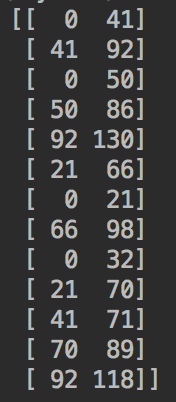
\includegraphics[scale=0.8]{lists}
\end{figure}

\subsection{Producing the Gantt chart}

\newpage
\section{Main Solution Code}

The code in \textit{solution\_final.py} contains the main program which carries out the process outlined by the question, i.e modelling the process of the cars moving across the city of Rome using the rules described. I have added scripts \textit{solution\_epsilon0.py} and \textit{solution\_accident\_occurs} to help answer the related questions at the end of the project.
\newline

Below are the imports used by the main program.

\begin{python}
# Imports
import numpy as np
import csv
import sys
import math as ma

# This import is needed for the last question
from solution_accident_occurs import max_index_tracker_no30
\end{python}

the variable \textit{max\_index\_tracker\_no30} is imported from another python script, 
\newline
\textit{solution\_accident\_occurs.py} in order to answer one of the questions. This will be discussed in detail later.
\leavevmode
\newline

Below are the functions required by the program. The docstring's explain their use.\
note: I will explain the use of the function away\_from\_52 properly later in the document.

\leavevmode
\newline

\begin{python}
# ------------------------------------------------------------------
# ------------------    FUNCTIONS USED     -------------------------
# ------------------------------------------------------------------

def calcWei(RX, RY, RA, RB, RV):
    """
    This function is taken from Tutorials. It calculates the weight matrix
    given information about each node in the system.
    :param RX: The x coordinates of each node in the system
    :param RY: The y coordinates of each node in the system
    :param RA: the connectivity of each node in the system
    :param RB: the connectivity of each node in the system
    :param RV: the speed limits across each edge in the system
    :return: usable weight matrix
    """

    n = len(RX)
    wei = np.zeros((n, n), dtype=float)
    m = len(RA)
    for i in range(m):
        xa = RX[RA[i] - 1]
        ya = RY[RA[i] - 1]
        xb = RX[RB[i] - 1]
        yb = RY[RB[i] - 1]
        dd = ma.sqrt((xb - xa) ** 2 + (yb - ya) ** 2)
        tt = dd / RV[i]
        wei[RA[i] - 1, RB[i] - 1] = tt
    return wei
    
def Dijkst(ist, isp, wei):
    """
    This Dijkstra's algorithm implementation is taken from tutorials.
    
    :param ist: the index of the starting node
    :param isp: the index of the node to reach
    :param wei: the assosciated weight matrix
    :return: 
    """

    # exception handling (start = stop)
    if ist == isp:
        shpath = [ist]
        return shpath

    # initialization
    N = len(wei)
    Inf = sys.maxint
    UnVisited = np.ones(N, int)
    cost = np.ones(N) * 1.e6
    par = -np.ones(N, int) * Inf

    # set the source point and get its (unvisited) neighbors
    jj = ist
    cost[jj] = 0
    UnVisited[jj] = 0
    tmp = UnVisited * wei[jj, :]
    ineigh = np.array(tmp.nonzero()).flatten()
    L = np.array(UnVisited.nonzero()).flatten().size

    # start Dijkstra algorithm
    while (L != 0):
        # step 1: update cost of unvisited neighbors,
        #         compare and (maybe) update
        for k in ineigh:
            newcost = cost[jj] + wei[jj, k]
            if (newcost < cost[k]):
                cost[k] = newcost
                par[k] = jj

        # step 2: determine minimum-cost point among UnVisited
        #         vertices and make this point the new point
        icnsdr = np.array(UnVisited.nonzero()).flatten()
        cmin, icmin = cost[icnsdr].min(0), cost[icnsdr].argmin(0)
        jj = icnsdr[icmin]

        # step 3: update "visited"-status and determine neighbors of new point
        UnVisited[jj] = 0
        tmp = UnVisited * wei[jj, :]
        ineigh = np.array(tmp.nonzero()).flatten()
        L = np.array(UnVisited.nonzero()).flatten().size

    # determine the shortest path
    shpath = [isp]
    while par[isp] != ist:
        shpath.append(par[isp])
        isp = par[isp]
    shpath.append(ist)

    return shpath[::-1]

def next_node(path):
    """ Returns the next index (after the node itself) in the path.
        If the path contains only one node, returns the node itself.
    """
    if len(path) == 1:
        return path[0]
    else:
        return path[1]


def update_weight_matrix(epsilon, c, original_weight_matrix, noNodes=58):
    """
    This function updates the weight matrix according to step 5 of the
    Project. Note the added fix - the weight matrix is not changed if
    the original entry was 0.



    :param epsilon: given in question
    :param c: the vector containing number of cars at each node
    :param original_weight_matrix: the weight matrix given by RomeEdges
    :param noNodes: number of nodes in the system
    :return: the updated weight matrix
    """
    new_weight_matrix = np.zeros((noNodes, noNodes))
    for i in range(noNodes):
        for j in range(noNodes):
            if original_weight_matrix[i, j] != float(0):
                new_weight_matrix[i, j] = original_weight_matrix[i, j] + \
                                          (epsilon * (float(c[i]) +
                                                      float(c[j]))) / float(2)
    return new_weight_matrix


def extract_data():
    """
    This function opens the RomeVertices and RomeEdges files, and creates
    global variables RomeX, RomeY, RomeA, RomeB and RomeV. These are variables
    used to create the original weight matrix.

    """
    global RomeX, RomeY, RomeA, RomeB, RomeV
    RomeX = np.empty(0, dtype=float)
    RomeY = np.empty(0, dtype=float)
    with open('./data/RomeVertices', 'r') as file:
        AAA = csv.reader(file)
        for row in AAA:
            RomeX = np.concatenate((RomeX, [float(row[1])]))
            RomeY = np.concatenate((RomeY, [float(row[2])]))
    file.close()
    RomeA = np.empty(0, dtype=int)
    RomeB = np.empty(0, dtype=int)
    RomeV = np.empty(0, dtype=float)
    with open('./data/RomeEdges2', 'r') as file:
        AAA = csv.reader(file)
        for row in AAA:
            RomeA = np.concatenate((RomeA, [int(row[0])]))
            RomeB = np.concatenate((RomeB, [int(row[1])]))
            RomeV = np.concatenate((RomeV, [float(row[2])]))
    file.close()
    
def away_from_52(edge):
    """
    Tells you whether a given edge is pointing completely away from
    node 52, in both the x and y directions.
    :param edge: an edge of the form [a,b]
    :return: boolean whether or not this points to or away from 52
    """

    # extract data for access to global variables
    extract_data()

    # the edge is of the form [a,b]
    a = edge[0]
    b = edge[1]

    # use RomeX and RomeY to find the coordinates for a,b and node 52.
    a_coord = [RomeX[a - 1], RomeY[a - 1]]
    b_coord = [RomeX[b - 1], RomeY[b - 1]]
    coord52 = [RomeX[51], RomeY[51]]

    # find the change in x/y from a -> b
    x_change = b_coord[0] - a_coord[0]
    y_change = b_coord[1] - a_coord[1]

    # find the change in x/y from a -> 52
    x_changeTo52 = coord52[0] - a_coord[0]
    y_changeto52 = coord52[1] - a_coord[1]

    # if we're at 52 we're moving away from it
    if a == 52:
        return True

    # if both point in same direction, false.
    if (x_changeTo52 > 0) and (x_change > 0):
        return False
    elif (x_changeTo52 < 0) and (x_change < 0):
        return False

    # if both point in same direction, false.
    if (y_changeto52 > 0) and (y_change > 0):
        return False
    elif (y_changeto52 < 0) and (y_change < 0):
        return False

    # all other tests have passed, so must be True.
    return True
\end{python}



Now using these functions, we can execute the main program.

\begin{python}
    # --------------------------------------------------------------
    # ------------------    Main program     -----------------------
    # --------------------------------------------------------------


if __name__ == '__main__':

    # Import the rome edges file
    extract_data()

    # Use the calcWei function from tutorials, along with the data set given
    # to calculate the weight matrix. Also create a copy which is the
    # temporary weight matrix.
    weight_matrix = misc.calcWei(RomeX, RomeY, RomeA, RomeB, RomeV)
    temp_wei = weight_matrix.copy()

    # Initialise minutes and number of nodes
    minutes = 200
    total_nodes = weight_matrix.shape[0]

    # Need a vector carNumbers which stores the number of cars at each vertex
    # in the graph.
    cars_at_node = np.zeros(total_nodes, dtype=int)
    cars_at_node_updated = cars_at_node.copy()  # cars_at_node updated is similar
    max_cars_at_node = cars_at_node.copy()  # max_cars_at_node is similar

    # To find the edges utilised, we need a 58x58 matrix of
    # False's. We will set each element to True if we move
    # cars from node i to node j.
    edge_utilised = np.zeros((total_nodes, total_nodes), dtype=bool)

    # Iterate through the 200 minutes
    for i in range(minutes):

        # Apply Dijkstra's algorithm to find the fastest path to node 52 in
        # the system. Then use next_node to find the next node in the given
        # path. (step 1)
        next_nodes = [next_node(Dijkst(node, 51, temp_wei))
                      for node in range(total_nodes)]

        # Move all cars as in steps 2,3. Iterate through every node in the
        # system to do this.
        for j_node in range(total_nodes):

            if j_node == 51:
                # We remove 40% of cars from node 52.
                cars_at_node_updated[51] += int(round(cars_at_node[51] * 0.6))
            else:

                # Initialise the number of cars at node j_node.
                number_of_cars = cars_at_node[j_node]

                # Initialise the next node to move to.
                node_to_move_to = next_nodes[j_node]

                # 70% of cars will move. to keep the total conserved, 
                # the amount staying is just 
                # number_of_cars - amount_moving
                amount_moving = int(round(0.7 * number_of_cars))
                amount_staying = number_of_cars - amount_moving

                # We now update cars_at_node.
                cars_at_node_updated[j_node] += amount_staying
                cars_at_node_updated[node_to_move_to] += amount_moving

                if amount_moving > 0:
                    # Update edges_utilised matrix
                    edge_utilised[j_node, node_to_move_to] = True

        # Now all cars have moved where they need to, we set cars_at_node
        # to this updated vector, and empty the updated vector for the next
        # iteration.
        cars_at_node = cars_at_node_updated.copy()
        cars_at_node_updated = np.zeros(total_nodes, dtype=int)

        # For the first 180 minutes, 20 cars are injected into node 13.
        if i <= 179:
            cars_at_node[12] += 20

        # The temporary weight matrix is updated.
        temp_wei = update_weight_matrix(0.01, cars_at_node, weight_matrix)

        # We have finished an iteration.

       # Now we calculate the maximum number of cars at each node in the system.
        max_cars_at_node = [max(cars_at_node[node], max_cars_at_node[node]) 
                            for node in range(total_nodes)]
\end{python}

\section{Questions}
\begin{enumerate}
\item \textbf{Determine for each node the maximum load (maximum number of cars) over the 200 iterations.}
\newline

As we have already incorporated the calculation of maximums in the loop, this is easy:

\begin{python}
max_index_tracker = [[node+1, max_cars_at_node[node]]
                         for node in range(total_nodes)]
\end{python}

Thus the i'th element of this array gives [node i, maximum number of cars of node i over the 200 iterations ]. The code to print is below along with the output.

\begin{python}
print('max_index_tracker is')
print(max_index_tracker[0:10])
print(max_index_tracker[10:20])
print(max_index_tracker[20:30])
print(max_index_tracker[30:40])
print(max_index_tracker[40:50])
print(max_index_tracker[50:(len(max_index_tracker)+1)])
\end{python}

\begin{figure}[h]
\caption{output of maximum loads}
\centering

\end{figure}

\item \textbf{Which are the five most congested nodes?} \newline
Given this array \textit{max\_index\_tracker}, we can simply sort by the second argument to find the top five most congested nodes
\begin{python}
top_five = sorted(max_index_tracker,
                      key=lambda node_and_max: -1 * node_and_max[1])[:5]
print('the five most congested nodes are')
print(top_five)
\end{python}

\begin{figure}[h]
\caption{top five most congested nodes output}
\centering

\end{figure}

In other words, the top five most congested nodes (from highest to lowest) is node 52 with 63 cars, node 25 with 40 cars, node 21 with 38 cars, node 30 with 32 cars and node 43 with 31 cars.
\newline


\item \textbf{Which edges are not utilized at all? Why?}
\leavevmode
\newline

In the main program we defined a 58x58 boolean matrix of False's, where throughout the process if cars moved from index i to index j, we made the [i,j] element of the matrix True.
\leavevmode
\newline

Thus, we have a matrix where indices (corresponding to edges) are \textit{True} if they are traversed by some amount of cars ($ > 0$) in the 200 minute process.
\leavevmode
\newline

All that is left to do is count the number of False's, making sure that we don't count a False if the edge couldn't be traversed to begin with (in the original weight matrix). This corresponds to an element of the original weight matrix being 0.

\begin{python}
# create a boolean matrix that corresponds to the condition
# described above
non_utilised_edges_matrix = (weight_matrix != float(0)) \
                                & (np.logical_not(edge_utilised))
                                
non_utilised_edges = [[i+1, j+1] for i in range(total_nodes)
                          for j in range(total_nodes)
                          if non_utilised_edges_matrix[i, j]]

\end{python}

So an element $[l,m]$ belonging to this vector \textit{non\_utilised\_edges} implies that the edge $l \to m$ is not utilised.

The code to print this and the output is below.

\begin{python}
print('the non utilised edges are')
print(non_utilised_edges[0:10])
print(non_utilised_edges[10:20])
print(non_utilised_edges[20:30])
print(non_utilised_edges[30:40])
print(non_utilised_edges[40:50])
print(non_utilised_edges[50:60])
print(non_utilised_edges[60:(len(non_utilised_edges)+1)])
\end{python}

\begin{figure}[h]
\caption{list of non utilised edges output}
\centering

\end{figure}

Now I answer \textit{why} these edges aren't utilised. 


For the vast majority of unused edges, it is intuitively clear that the reason they are included is because they are pointing completely away from the direction towards node 52. For example, I have highlighted edges $4 \to 1$, $12 \to 4$ and $52 \to 58$ in figure 3.4.

\begin{figure}[h]
\caption{City of Rome graph map with drawn edges}
\centering

\end{figure}
 
These edges in particular are not only in the wrong in the x direction, but wrong in the y direction too. I have created the function \textit{away\_from\_52} below to return a boolean depending on whether a given edge is pointing completely away from node 52. i.e. in both x and y direction.

\leavevmode
\newline
\leavevmode
\newline



\begin{python}
def away_from_52(edge):
    """
    Tells you whether a given edge is pointing completely away from
    node 52, in both the x and y directions.
    :param edge: an edge of the form [a,b]
    :return: boolean whether or not this points to or away from 52
    """

    # extract data for access to global variables
    extract_data()

    # the edge is of the form [a,b]
    a = edge[0]
    b = edge[1]

    # use RomeX and RomeY to find the coordinates for a,b and node 52.
    a_coord = [RomeX[a - 1], RomeY[a - 1]]
    b_coord = [RomeX[b - 1], RomeY[b - 1]]
    coord52 = [RomeX[51], RomeY[51]]

    # find the change in x/y from a -> b
    x_change = b_coord[0] - a_coord[0]
    y_change = b_coord[1] - a_coord[1]

    # find the change in x/y from a -> 52
    x_changeTo52 = coord52[0] - a_coord[0]
    y_changeto52 = coord52[1] - a_coord[1]

    # if we're at 52 we're moving away from it
    if a == 52:
        return True

    # if both point in same direction, false.
    if (x_changeTo52 > 0) and (x_change > 0):
        return False
    elif (x_changeTo52 < 0) and (x_change < 0):
        return False

    # if both point in same direction, false.
    if (y_changeto52 > 0) and (y_change > 0):
        return False
    elif (y_changeto52 < 0) and (y_change < 0):
        return False

    # all other tests have passed, so must be True.
    return True  
\end{python}

We then run this to find the number of edges facing completely away from node 52.

\begin{python}
new_unused = list(non_utilised_edges)

for _, edge in enumerate(non_utilised_edges):
	if away_from_52(edge):
	new_unused.remove(edge)

print('length of new_unused is %i' % len(new_unused))
\end{python}

\begin{figure}[h]
\caption{length of new\_unused list}
\centering

\end{figure}

So out of 71 unused edges, 41 of them were facing completely away from node 52. In a similar way we can remove nodes that are facing away from node 52 in the x direction only. 

I print the remaining edges below

\begin{python}
    print(new_unused[0:10])
    print(new_unused[10:20])
    print(new_unused[20:31])
\end{python}

\begin{figure}[h]
\caption{list of unused edges that aren't facing completely away from node 52}
\centering
\end{figure}



We note that from the first question where we found the maximum load for all cars over the 200 iterations, it is clear that nodes with maximum load 0 (i.e. node 3, 5, 8 etc) will always appear on this list since they were never visited. However, the real question is \textit{why} they were never visited. \\

If we perform Dijkstra's algorithm on the original weight matrix and find the fastest route form node 13 to 52, we find this:

\begin{python}
print(Dijkst(12,51,weight_matrix))
\end{python}

\begin{figure}[h]
\caption{Dijkstra's algorithm path from 13 to 52 (python indices)}
\centering

\end{figure}

\begin{figure}[h]
\caption{Dijkstra's algorithm path from 13 to 52 with constant weight matrix}
\centering

\end{figure}



note that these are the python indices and not the actual node numbers.

If we look at figure 3.8, this means without taking the effect of congestion, the fastest path throughout the city is almost completely at the bottom of the map, by the river. This means that it is unlikely for a car to need to travel through the upper west side of the city, such as through nodes 1,3,5 and 2. The only way the shortest path for a car could include such nodes is if the rest of the city is \textit{so} congested that the shortest path will indeed require these upper left nodes. We can see that edges like [3,2], [8,9] are not optimal for this reason, and are thus unused.

There are lots of edges that although aren't facing in the wrong direction in both the x and y direction, but will obviously never lead to an optimal solution. Such as [57,55] and [56,54]. This is because these nodes have a very small degree, 2 or 3. So if the optimal path runs through them (in the opposite direction), the other direction which tracks backwards will not be part of an optimal solution.

We can also consider the fact that if an edge is used by cars, the inverse of that edge is unlikely to be used again. This makes sense if we consider that 71 edges are unused out of a total of 156 edges (almost 1/2). So if we compare all the edges available to use and the edges unused, we should find a high correlation between pairs of the form [a,b] and [b,a] existing in either set. This is another reason highly used edges like [55,57] and [56,54] are not traversed in the opposite direction, as discussed in the paragraph above.

\item \textbf{What flow pattern do we observe for parameter $\epsilon = 0$?}

See the \textit{solution\_epsilon0.py} file. The main program is exactly the same, but for one change. I have replaced epsilon = 0.01 with epsilon = float(0) where we update the weight matrix in the main for loop.

\begin{python}
temp_wei = update_weight_matrix(float(0), cars_at_node, weight_matrix)
\end{python}

Now, if we consider the formula for the adjusted weight matrix at each iteration, where $w_{ij} = w_{ij}^{(0)} + \epsilon \frac{c_{i} + c_{j}}{2}$, we see that the weight matrix remains unchanged.

As discussed in lectures, Dijkstra's algorithm is an example of a greedy algorithm. Since the time discrete process we are modelling uses Dijkstra's algorithm one node at a time (with the same weight matrix), we know that the shortest path from node 13 to node 52 will remain constant throughout the process.

Furthermore, let P be a node on the shortest path between node 13 and 52,

$$ 13 \to .. \to \ P \to p_{1} \to ... \to p_{n-1} \to 52 $$

Then the shortest path from node P to node 52 is 

$$ P \to p_{1} \to ... \to p_{n-1} \to 52 $$

Since the weight matrix is unchanged. If the shortest path between node P and node 52 were anything else then the shortest path between node 13 and node 52 would not be $13 \to ... \to P \to p_{1} \to ... \to p_{n-1} \to 52$.

In other words, finding the shortest path from node to node with a constant weight matrix is the same as finding the overall shortest path using the same weight matrix. We can simply use the utilised edges to see that the flow of cars in the system follows this path. Printing the cars\_at\_node vector throughout the 200 minutes verifies this.

\begin{python}
# regular dijkstra's path
print('the Dijkstra\'s path is ')
print(dijk.Dijkst(12, 51, weight_matrix))

utilised_edges = [[i, j] for i in range(noNodes) 
                  for j in range(noNodes) 
                  if edge_utilised[i, j]] # this matrix is defined in the main 
                  			       #code
print('the utilised edges are')
print(utilised_edges)
\end{python}

\begin{figure}[h]
\caption{Dijkstra's path with utilised edges output (both in Python indices for clarity)}
\centering

\end{figure}

Since all of these edges have a distinct head to tail connection, I can be sure the cars follow the path in the order we expect.


\item \textbf{An accident occurs at node 30 (python-index 29) which blocks any route to or from node 30. Which nodes are now the most congested and what is their maximum load? Which nodes (besides node 30) decrease the most in peak value, which nodes in- crease the most in peak value?}

See \textit{solution\_accident\_occurs.py}. The main code is exactly the same as before, but for these changes:

Since no car can reach node 30, we need to make the 30th row and 30th column of the weight matrix equal to 0s. 

\begin{python}
# Use the calcWei function from tutorials, along with the data set given
# to calculate the weight matrix. Also create a copy which is the
# temporary weight matrix.
weight_matrix = calcWei(RomeX, RomeY, RomeA, RomeB, RomeV)

# The accident at node 30 means that the 30th row and 30th column is all 0
weight_matrix[29, :] = np.zeros(58, dtype=float)
weight_matrix[:, 29] = np.zeros(58, dtype=float)

temp_wei = weight_matrix.copy()
\end{python}

Once we begin the for loop iterating through the 200 minutes, we compute the next nodes as before. But there is no path between node 30 and 52, so we add this "if node!=29" statement to the next\_nodes calculation.

We also insert a 0 at index 29, so the nodes align properly again.

\begin{python}
# Iterate through the 200 minutes
for i in range(minutes):

    # Apply Dijkstra's algorithm to find the fastest path to node 52 in
    # the system. Then use next_node to find the next node in the given
    # path. (step 1)
    next_nodes = [next_node(Dijkst(node, 51, temp_wei))
                  for node in range(total_nodes) if node != 29]

    next_nodes.insert(29, 29)  # send the 0 cars from 29 to itself
\end{python}

We can ignore node 30 when moving the cars through the system, so we add this else if statement.

\begin{python}
 for j_node in range(total_nodes):

        if j_node == 51:
            # We remove 40% of cars from node 52.
            cars_at_node_updated[51] += int(round(cars_at_node[51] * 0.6))
            # really, we can just ignore node 30.
        elif j_node != 29:
\end{python}

Now we create this variable max\_index\_tracker\_no30, which is simply the array of all the nodes with the maximum load they carry over the 200 iterations. This is then imported into the \textit{solution\_final.py} file as outlined before.

\begin{python}
# Find the top 5 most congested nodes.
max_index_tracker_no30 = [[node+1, max_cars_at_node[node]]
                          for node in range(total_nodes)]
\end{python}

Now, back in \textit{solution\_final.py} we compare and print the required values.

\begin{python}
top_eight = sorted(max_index_tracker_no30, 
                       key=lambda node_and_max: -1 * node_and_max[1])[:8]
print(top_eight)
\end{python}

These are the top 8 most congested nodes when node 30 is blocked.

\begin{figure}[h]
\caption{Top 8 most congested nodes with maximum loads when node 30 is blocked}
\centering

\end{figure}

\leavevmode
\newline



Now we find the nodes which increase/decrease the most in peak value.

\begin{python}
    differences = []
    for k in range(total_nodes):
        if k == 29:
            differences.append([k+1, 0])  # ignore when analysing
        else:
            differences.append([k+1, max_index_tracker[k][1] 
                                - max_index_tracker_no30[k][1]])

    sorted_differences_most = \
        sorted(differences, 
               key=lambda node_and_max: -1 * node_and_max[1])[:8]
    sorted_differences_least = \
        sorted(differences, 
               key=lambda node_and_max: node_and_max[1])[:8]
    print(sorted_differences_most)
    print(sorted_differences_least)
\end{python}

\begin{figure}[h]
\caption{The top 8 nodes which increased the most in peak value, followed by (next line) the top 8 nodes that decreased the most in peak value, all with their difference in peak values.}
\centering

\end{figure}

These elements represents the node number and the difference in maximum load from before to when node 30 is congested. So for example, node 6 increased its peak value by 5, and node 43 decreased its peak value by 14.



\end{enumerate}
\end{document}
